% !TeX root = ../thuthesis-example.tex

\chapter{持续集成与持续部署(CI/CD)的设计与实现}
\label{chap:mcp-tdd-cicd}

在现代软件工程中,CI/CD(持续集成与持续部署)已成为保障开发效率与代码质量的核心机制。传统搭建 CI/CD 流水线通常依赖人工配置脚本与手动部署流程,不仅繁琐易错,且难以在多工具协同开发场景中实现统一管理。

bolt.SE 通过模型上下文协议(MCP)引入标准化的工具接口,使大语言模型(LLM)能够自动访问如 GitHub、GitLab 等远程仓库管理平台,执行如创建仓库、推送代码、触发流水线等操作。一旦接入了具备 CI/CD 能力的 MCP 服务器(例如 \texttt{server-github} 或 \texttt{server-gitlab}),系统即具备了构建自动化部署流程的基础。

另一方面,bolt.SE 的测试驱动开发(TDD)模块提供从测试定义到代码验证的一体化支持,使 LLM 在开发早期即能生成具备行为保证的功能模块。二者结合,即形成测试定义、功能实现、代码验证、版本控制、自动部署的完整开发闭环。

本章将展示如何在 bolt.SE 中配置 GitLab MCP 工具,配合 TDD 流程构建 Todo 应用,并自动生成 CI/CD 配置,实现从本地测试到远程部署的全链路自动化流程。这一过程体现了 MCP 与 TDD 的协同机制如何系统性地提升 LLM 驱动开发的工程化能力。

实验流程首先由 Jest 测试用例反向生成最小可行代码并即时验证(TDD),随后通过 MCP 连接 server-gitlab,在 GitLab 上新建仓库并推送代码,最后由 LLM 自动编写 \texttt{.gitlab-ci.yml},为主干推送触发测试并部署到 Vercel。

\section{环境准备与整体流程}
\label{sec:cicd-overview}

\begin{figure}[H]
    \centering
    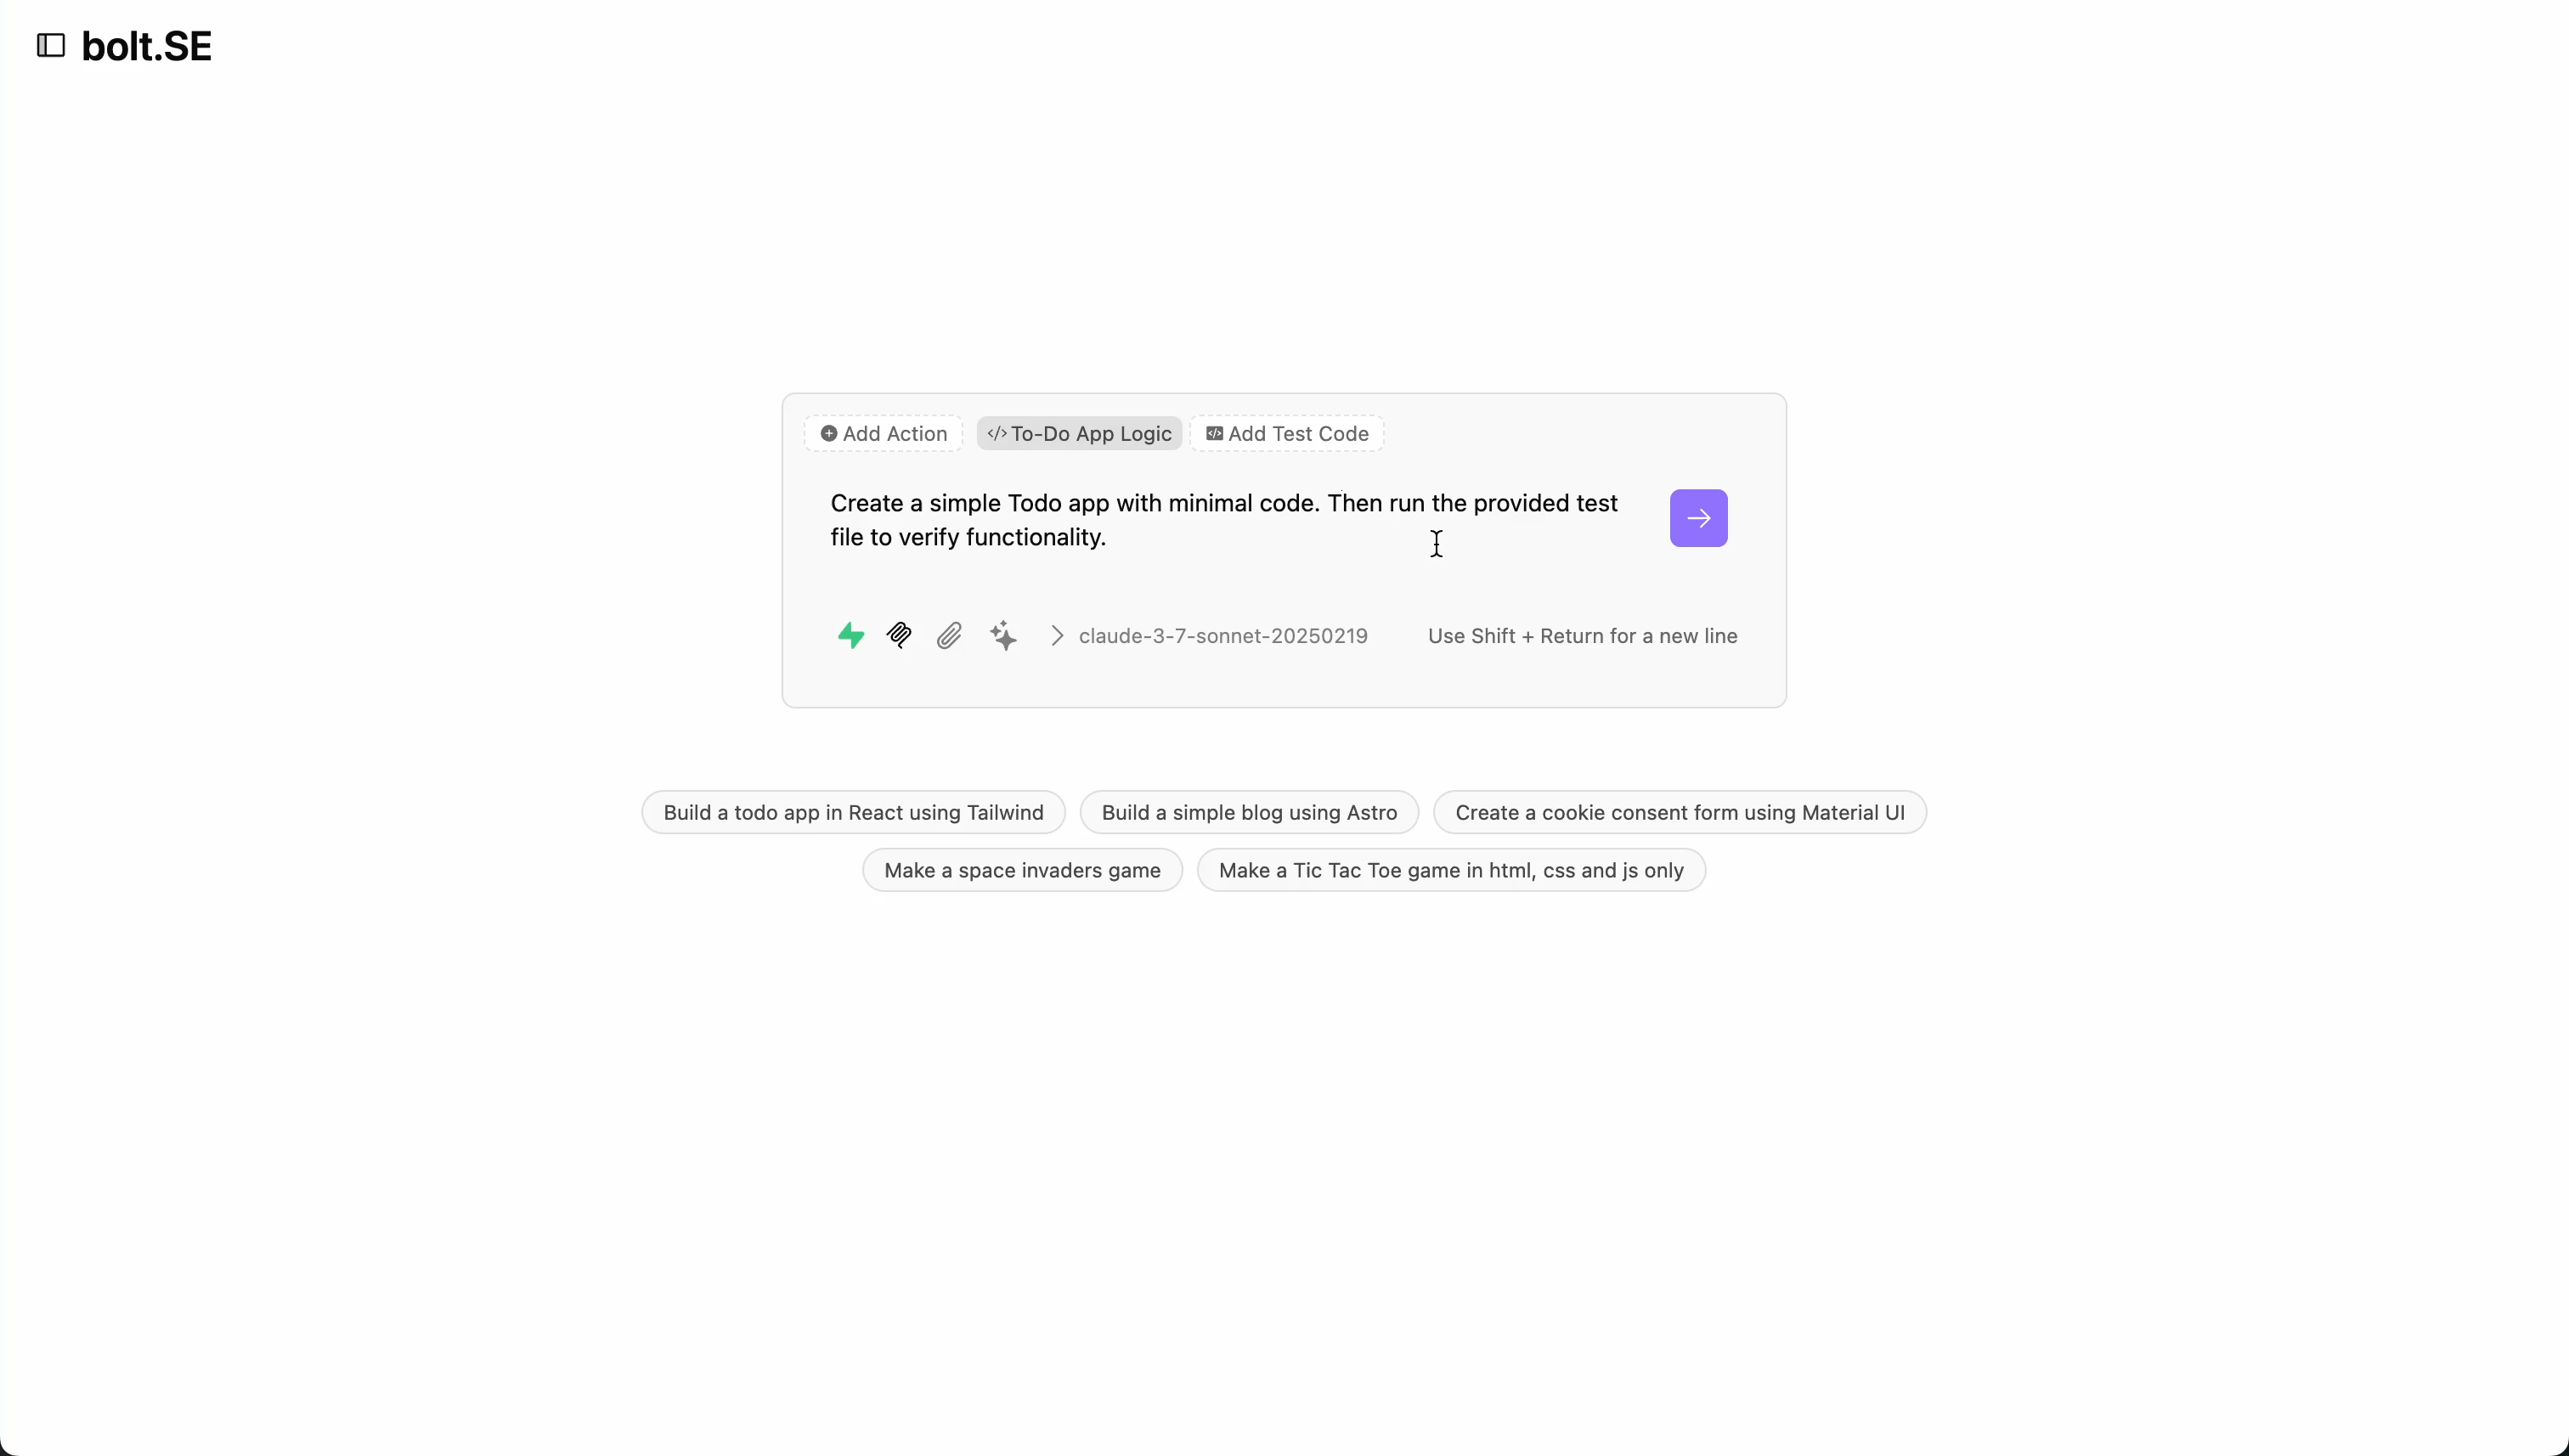
\includegraphics[width=\textwidth]{figures/screenshots/ci-cd/ci_prompt.png}
    \caption{开发者输入指令}
    \label{fig:ci_prompt}
\end{figure}

如图 \ref{fig:ci_prompt} 所示,开发者输入指令:"Create a simple Todo app with minimal code. Then run the provided test file to verify functionality."

系统即开始驱动以下流程:

\begin{itemize}
  \item 解析 Jest 测试,用于约束 LLM 生成代码(TDD 模块)
  \item 生成 React + Vite 工程、通过全部断言并预览界面
  \item 连接 \texttt{server-gitlab},验证令牌有效性(MCP 模块)
  \item 生成 \texttt{.gitlab-ci.yml}、\texttt{vercel.json} 等 CI 配置(LLM)
  \item 调用 \texttt{create\_repository} 工具,在 GitLab 创建远端仓库(MCP)
  \item 将本地文件推送至远端并触发首轮流水线
\end{itemize}

\section{配置 GitLab MCP 服务器}
\label{sec:cicd-mcp-config}

图 \ref{fig:mcp_gitlab_cfg} 展示了 \texttt{server-gitlab} 的 JSON 配置。  
要点如下:

\begin{itemize}
  \item 通过 \texttt{npx -y @modelcontextprotocol/server-gitlab} 启动本地转接进程,传输类型为 \texttt{stdio}。  
  \item 使用 \texttt{GITLAB\_PERSONAL\_ACCESS\_TOKEN} 环境变量完成 OAuth 认证,仅暴露最小权限作用域(\texttt{api\_read\_write})。  
  \item 再次点击 "Check availability" 后,状态变为 Available,客户端即可发现 \texttt{create\_repository}、\texttt{list\_projects} 等工具。  
\end{itemize}

\begin{figure}[H]
  \centering
  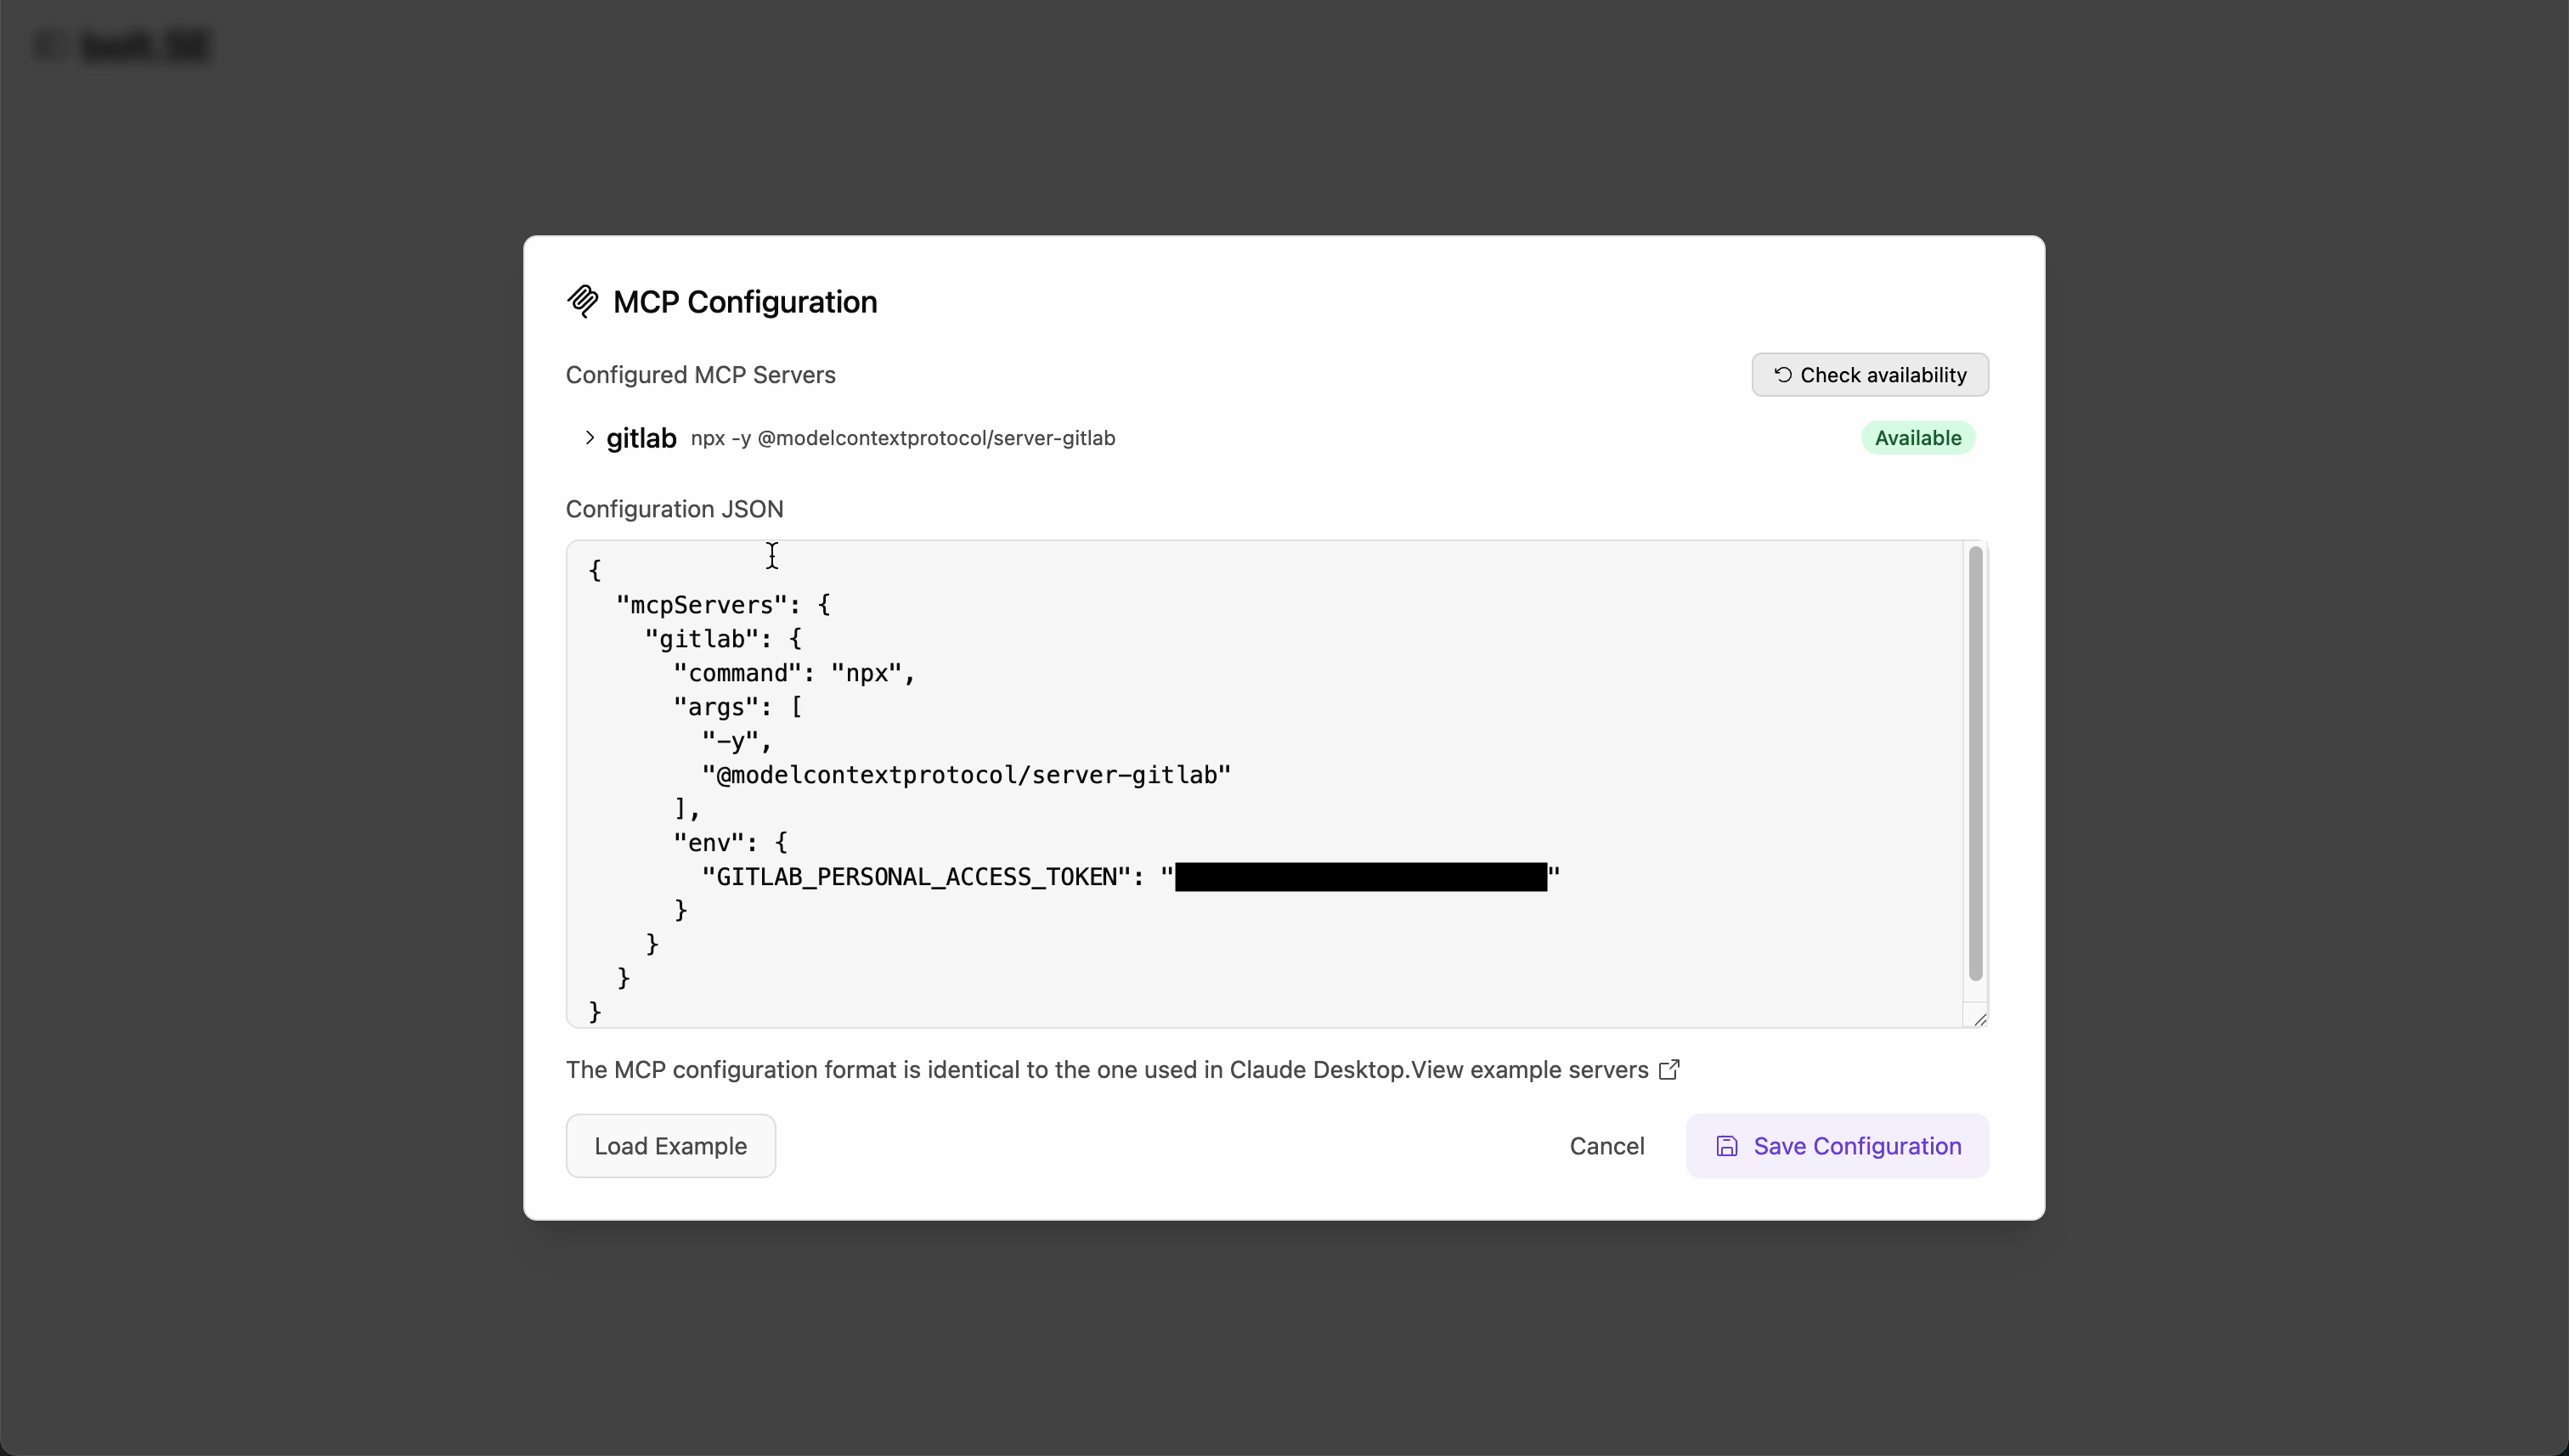
\includegraphics[width=\textwidth]{figures/screenshots/ci-cd/mcp_gitlab_cfg.png}
  \caption{MCP 服务器 \texttt{server-gitlab} 配置与连通性检测}
  \label{fig:mcp_gitlab_cfg}
\end{figure}

\section{导入 Jest 测试并生成应用代码}

开发者在 Add Test 模态框中粘贴 \texttt{to-do\_app\_logic.test.js}(图 \ref{fig:jest_import})。  
系统解析出四条断言:\textit{adds task}、\textit{rejects empty task}、\textit{toggles status}、\textit{deletes task}。  
随后,LLM 依据 TDD 原则生成最小实现;所有测试一次通过,且预览页展示可交互页面(图 \ref{fig:app_preview})。

\begin{figure}[H]
  \centering
  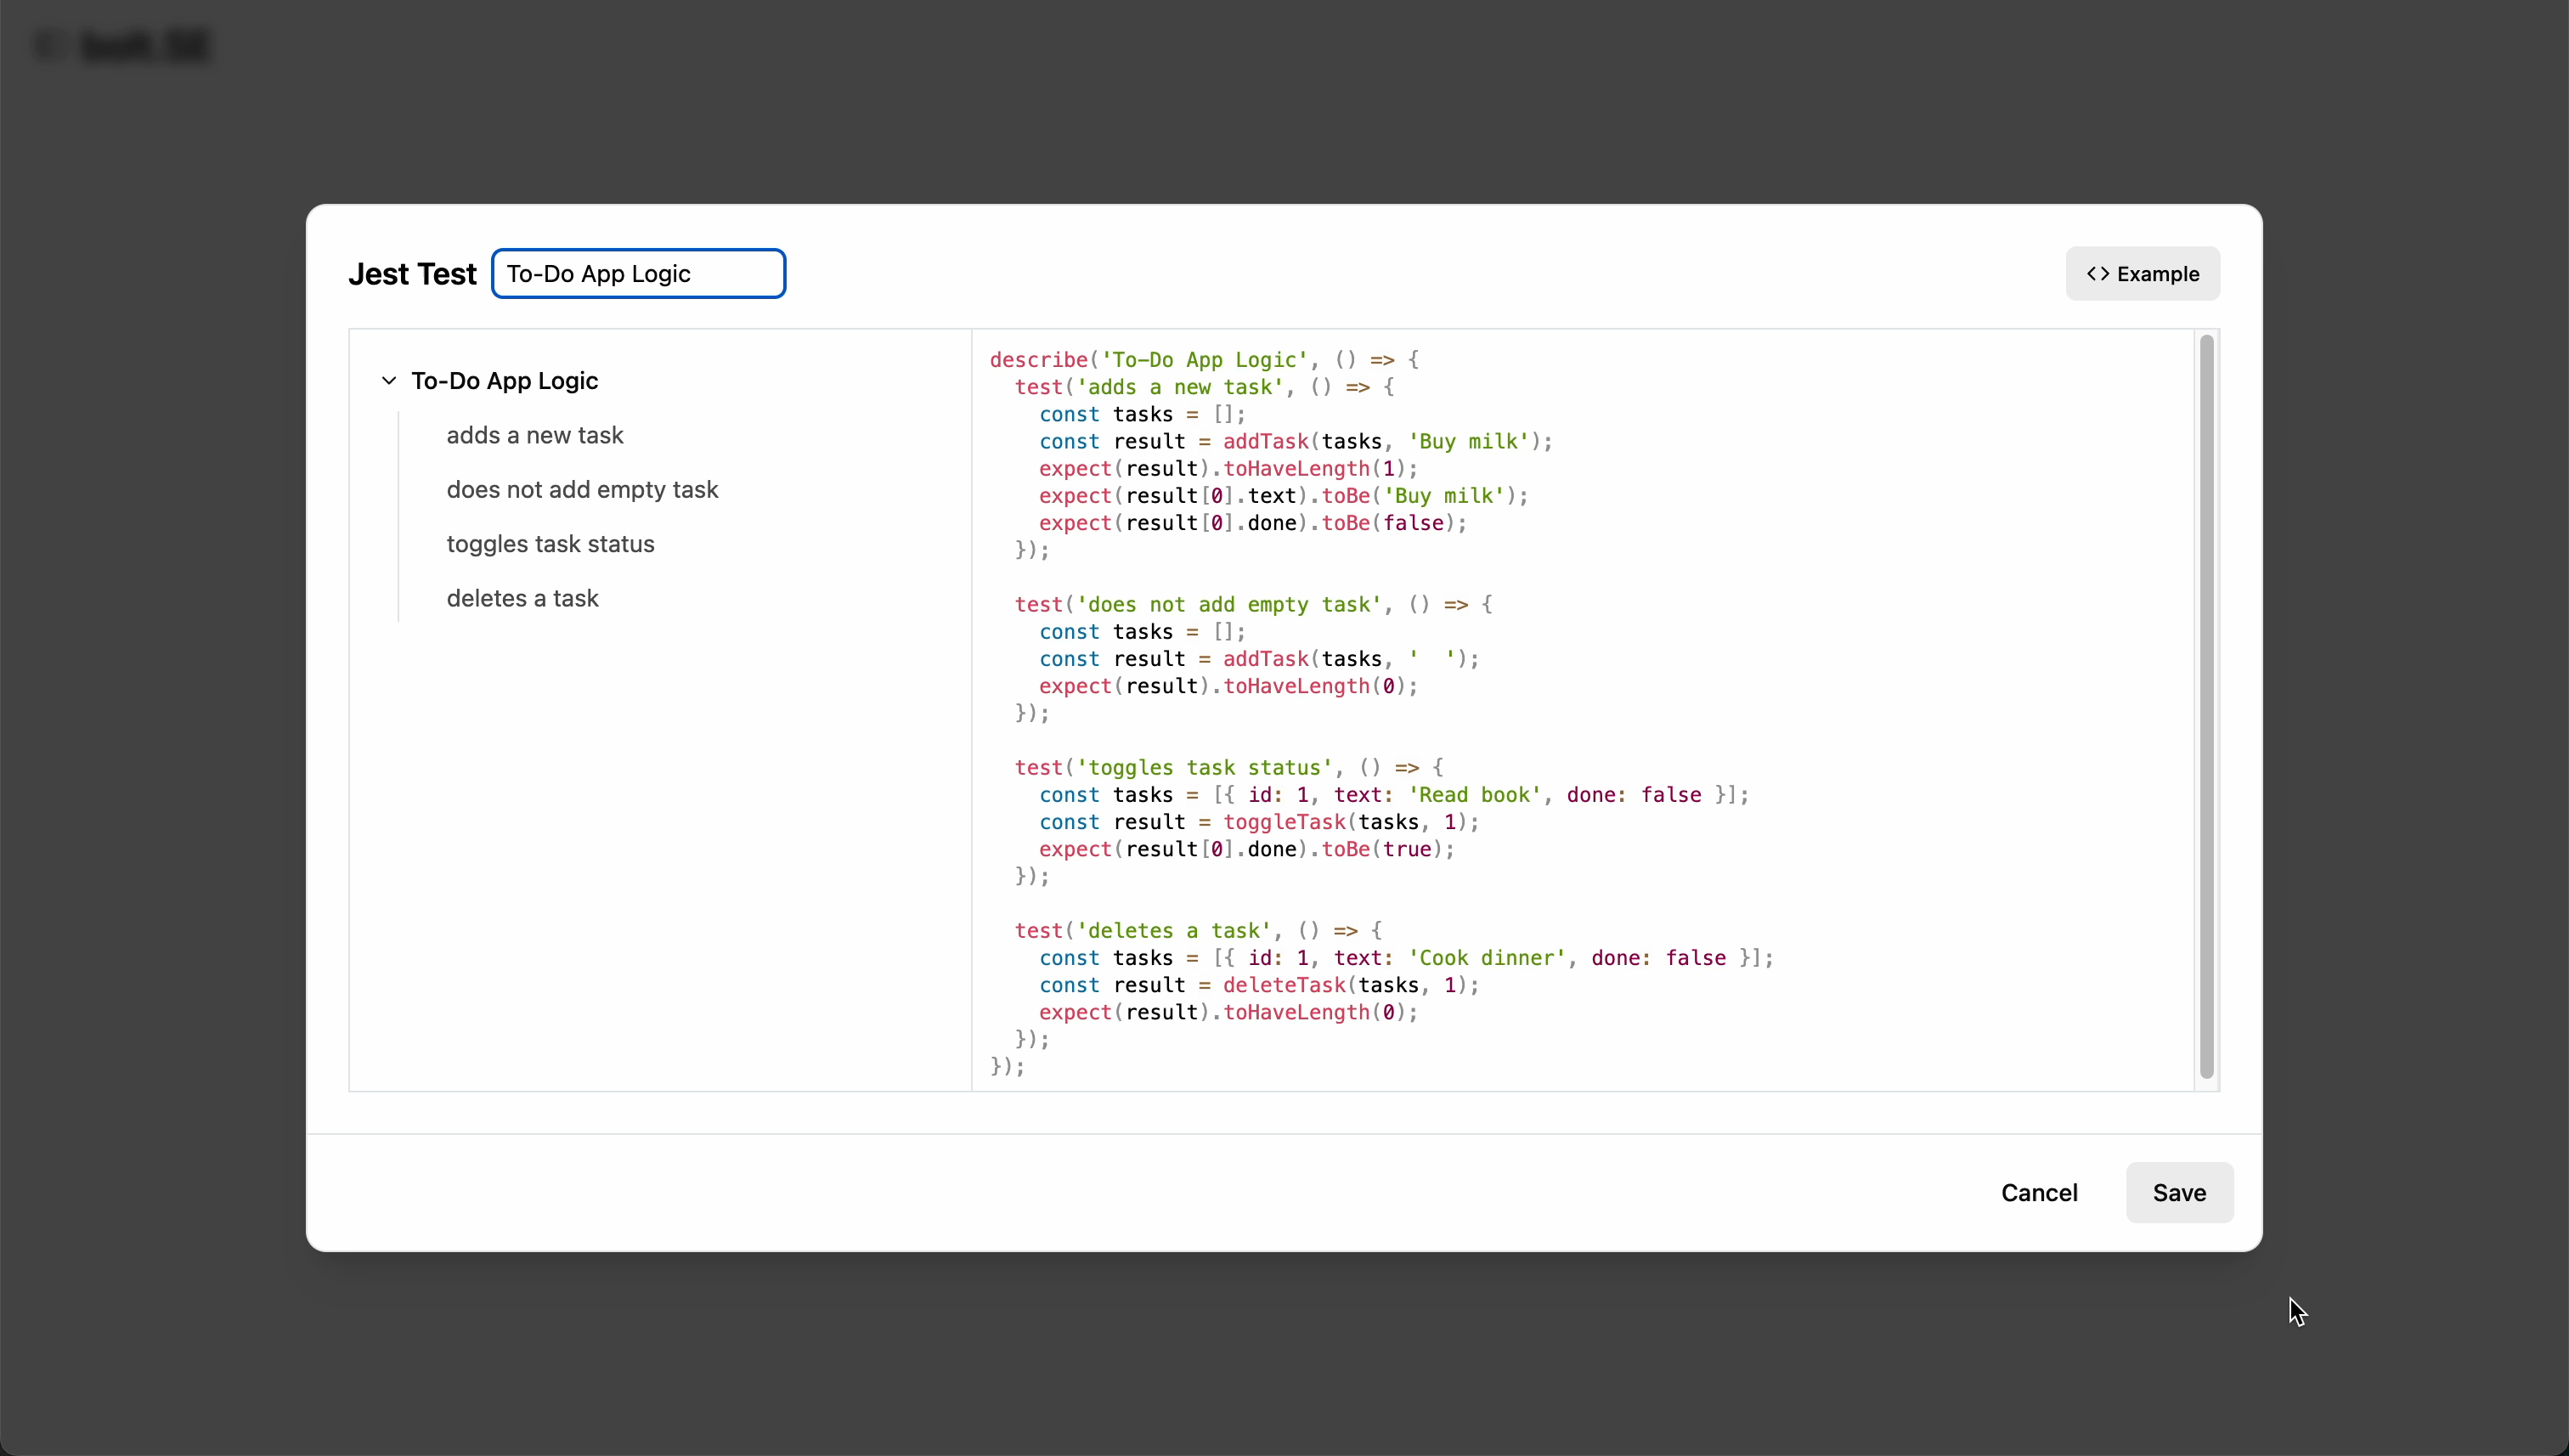
\includegraphics[width=\textwidth]{figures/screenshots/ci-cd/jest_import.png}
  \caption{导入 Jest 测试文件并解析测试树}
  \label{fig:jest_import}
\end{figure}

\begin{figure}[H]
  \centering
  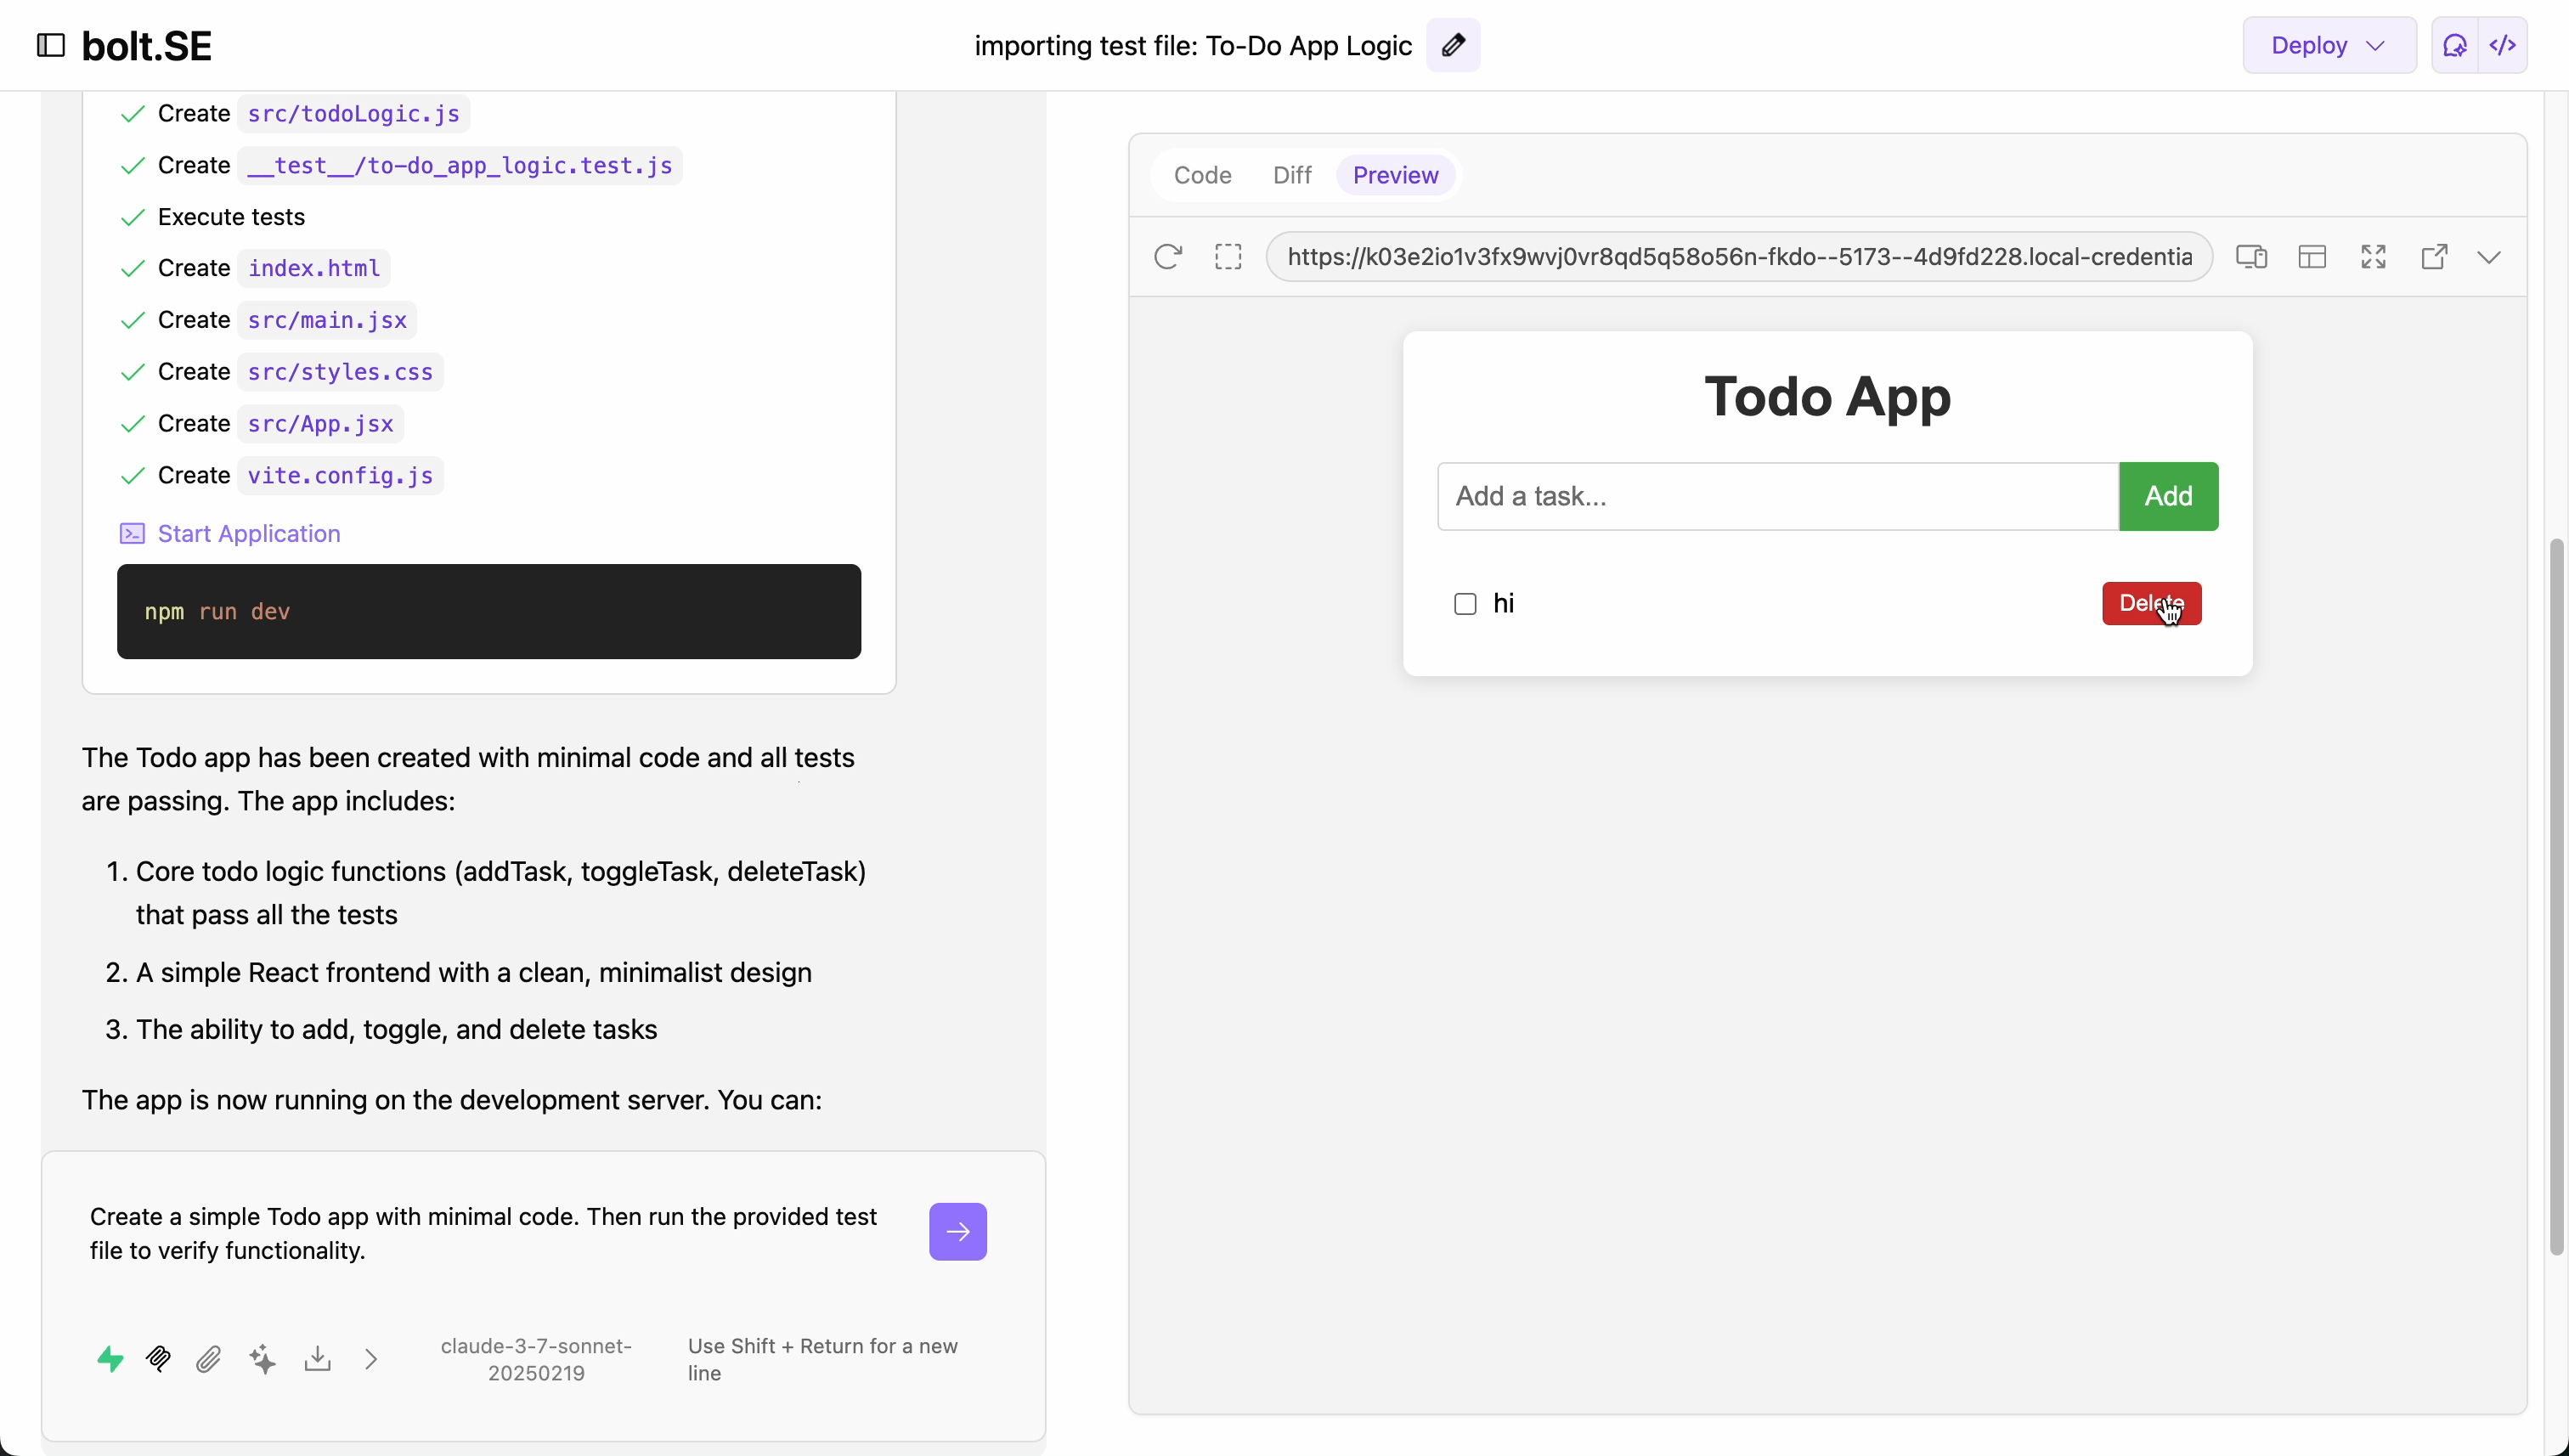
\includegraphics[width=.8\textwidth]{figures/screenshots/ci-cd/app_preview.png}
  \caption{全部测试通过后的运行预览}
  \label{fig:app_preview}
\end{figure}

\section{自动生成 GitLab CI 配置}
\label{sec:cicd-ci-yml}

LLM 接管流水线脚本编写,输出精简版 \texttt{.gitlab-ci.yml}(图 \ref{fig:ci_plan},左侧工作卡片)。核心逻辑包括:测试阶段使用 \texttt{node:18} 镜像,执行 \texttt{npm ci \&\& npm test};部署阶段仅当分支为 \texttt{main} 且测试成功时调用 Vercel CLI 部署;同时缓存 \texttt{node\_modules} 以加速后续执行。

\begin{figure}[H]
  \centering
  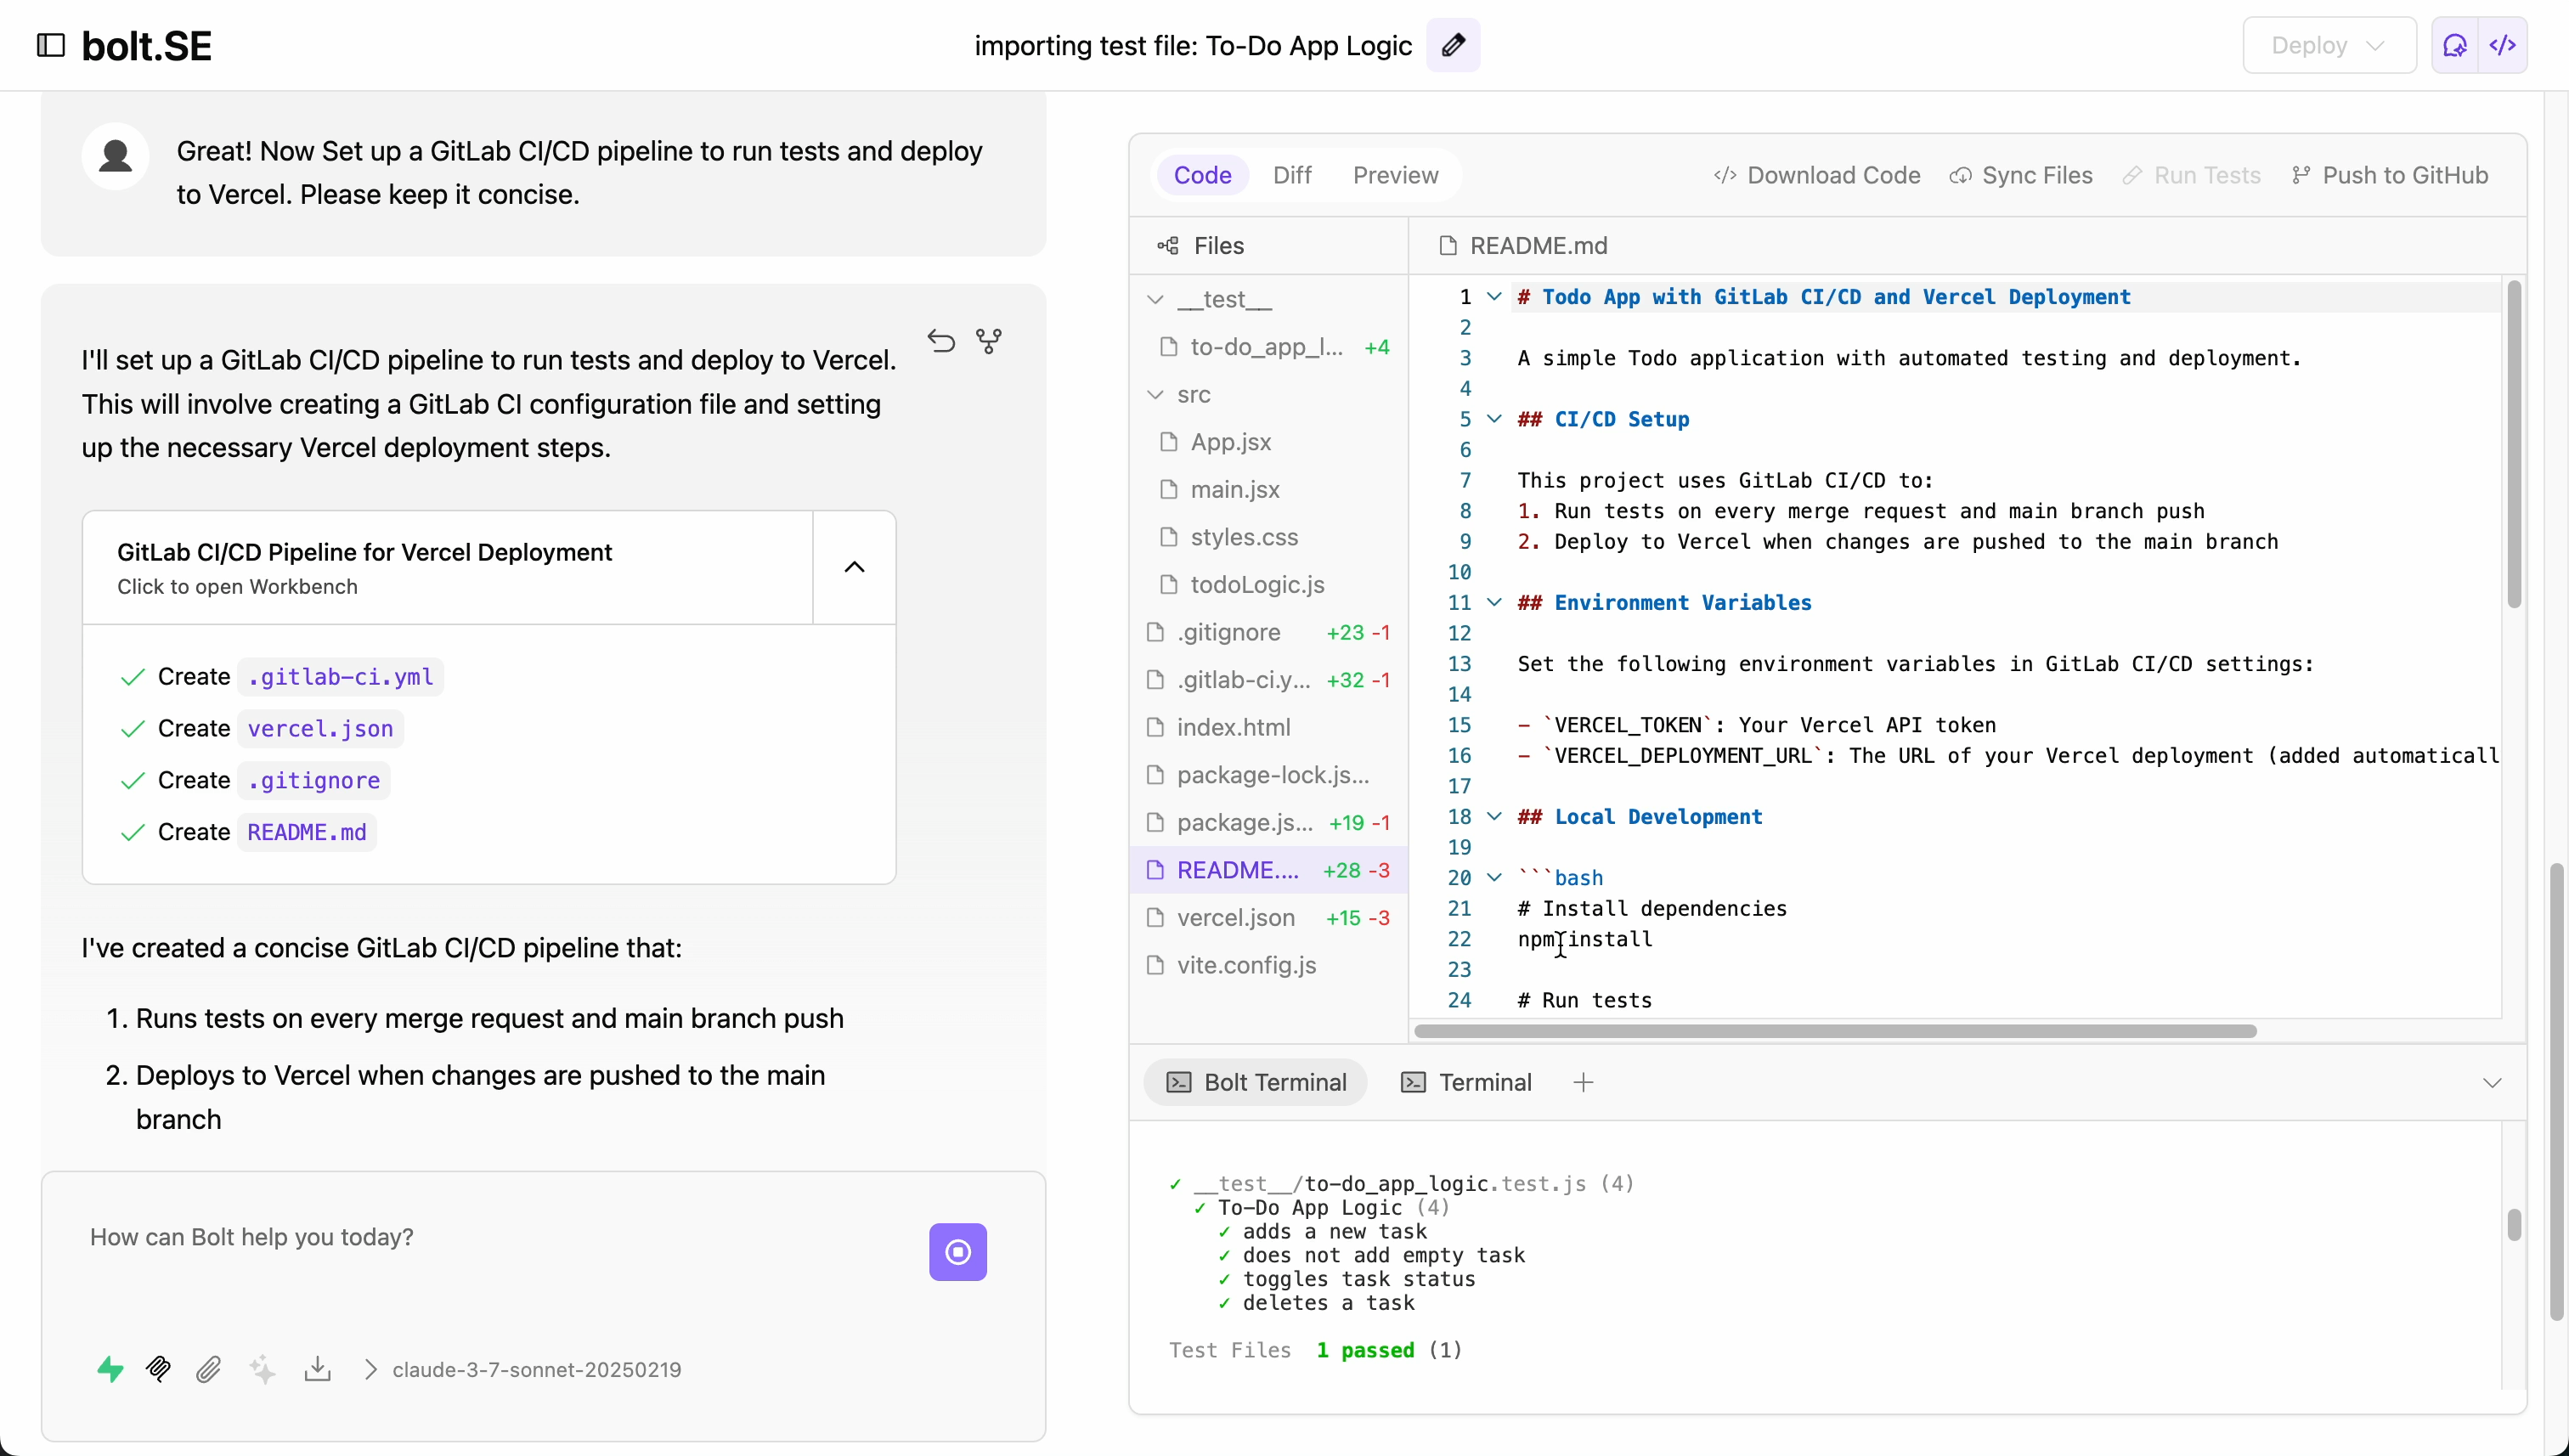
\includegraphics[width=\textwidth]{figures/screenshots/ci-cd/ci_plan.png}
  \caption{生成 CI/CD 计划卡片及 \texttt{.gitlab-ci.yml} 代码差异}
  \label{fig:ci_plan}
\end{figure}

\section{仓库初始化与首轮流水线触发}

系统调用 \texttt{create\_repository} 工具(图 \ref{fig:mcp_invocation}),自动在 GitLab 新建 \texttt{todo-app} 仓库并返回 HTTPS 地址。紧接着执行 Git 操作:将本地 Vite 工程全部推送至远端,并在 CI 界面自动触发 \texttt{npm test} 与 Vercel 部署作业。

\begin{figure}[H]
  \centering
  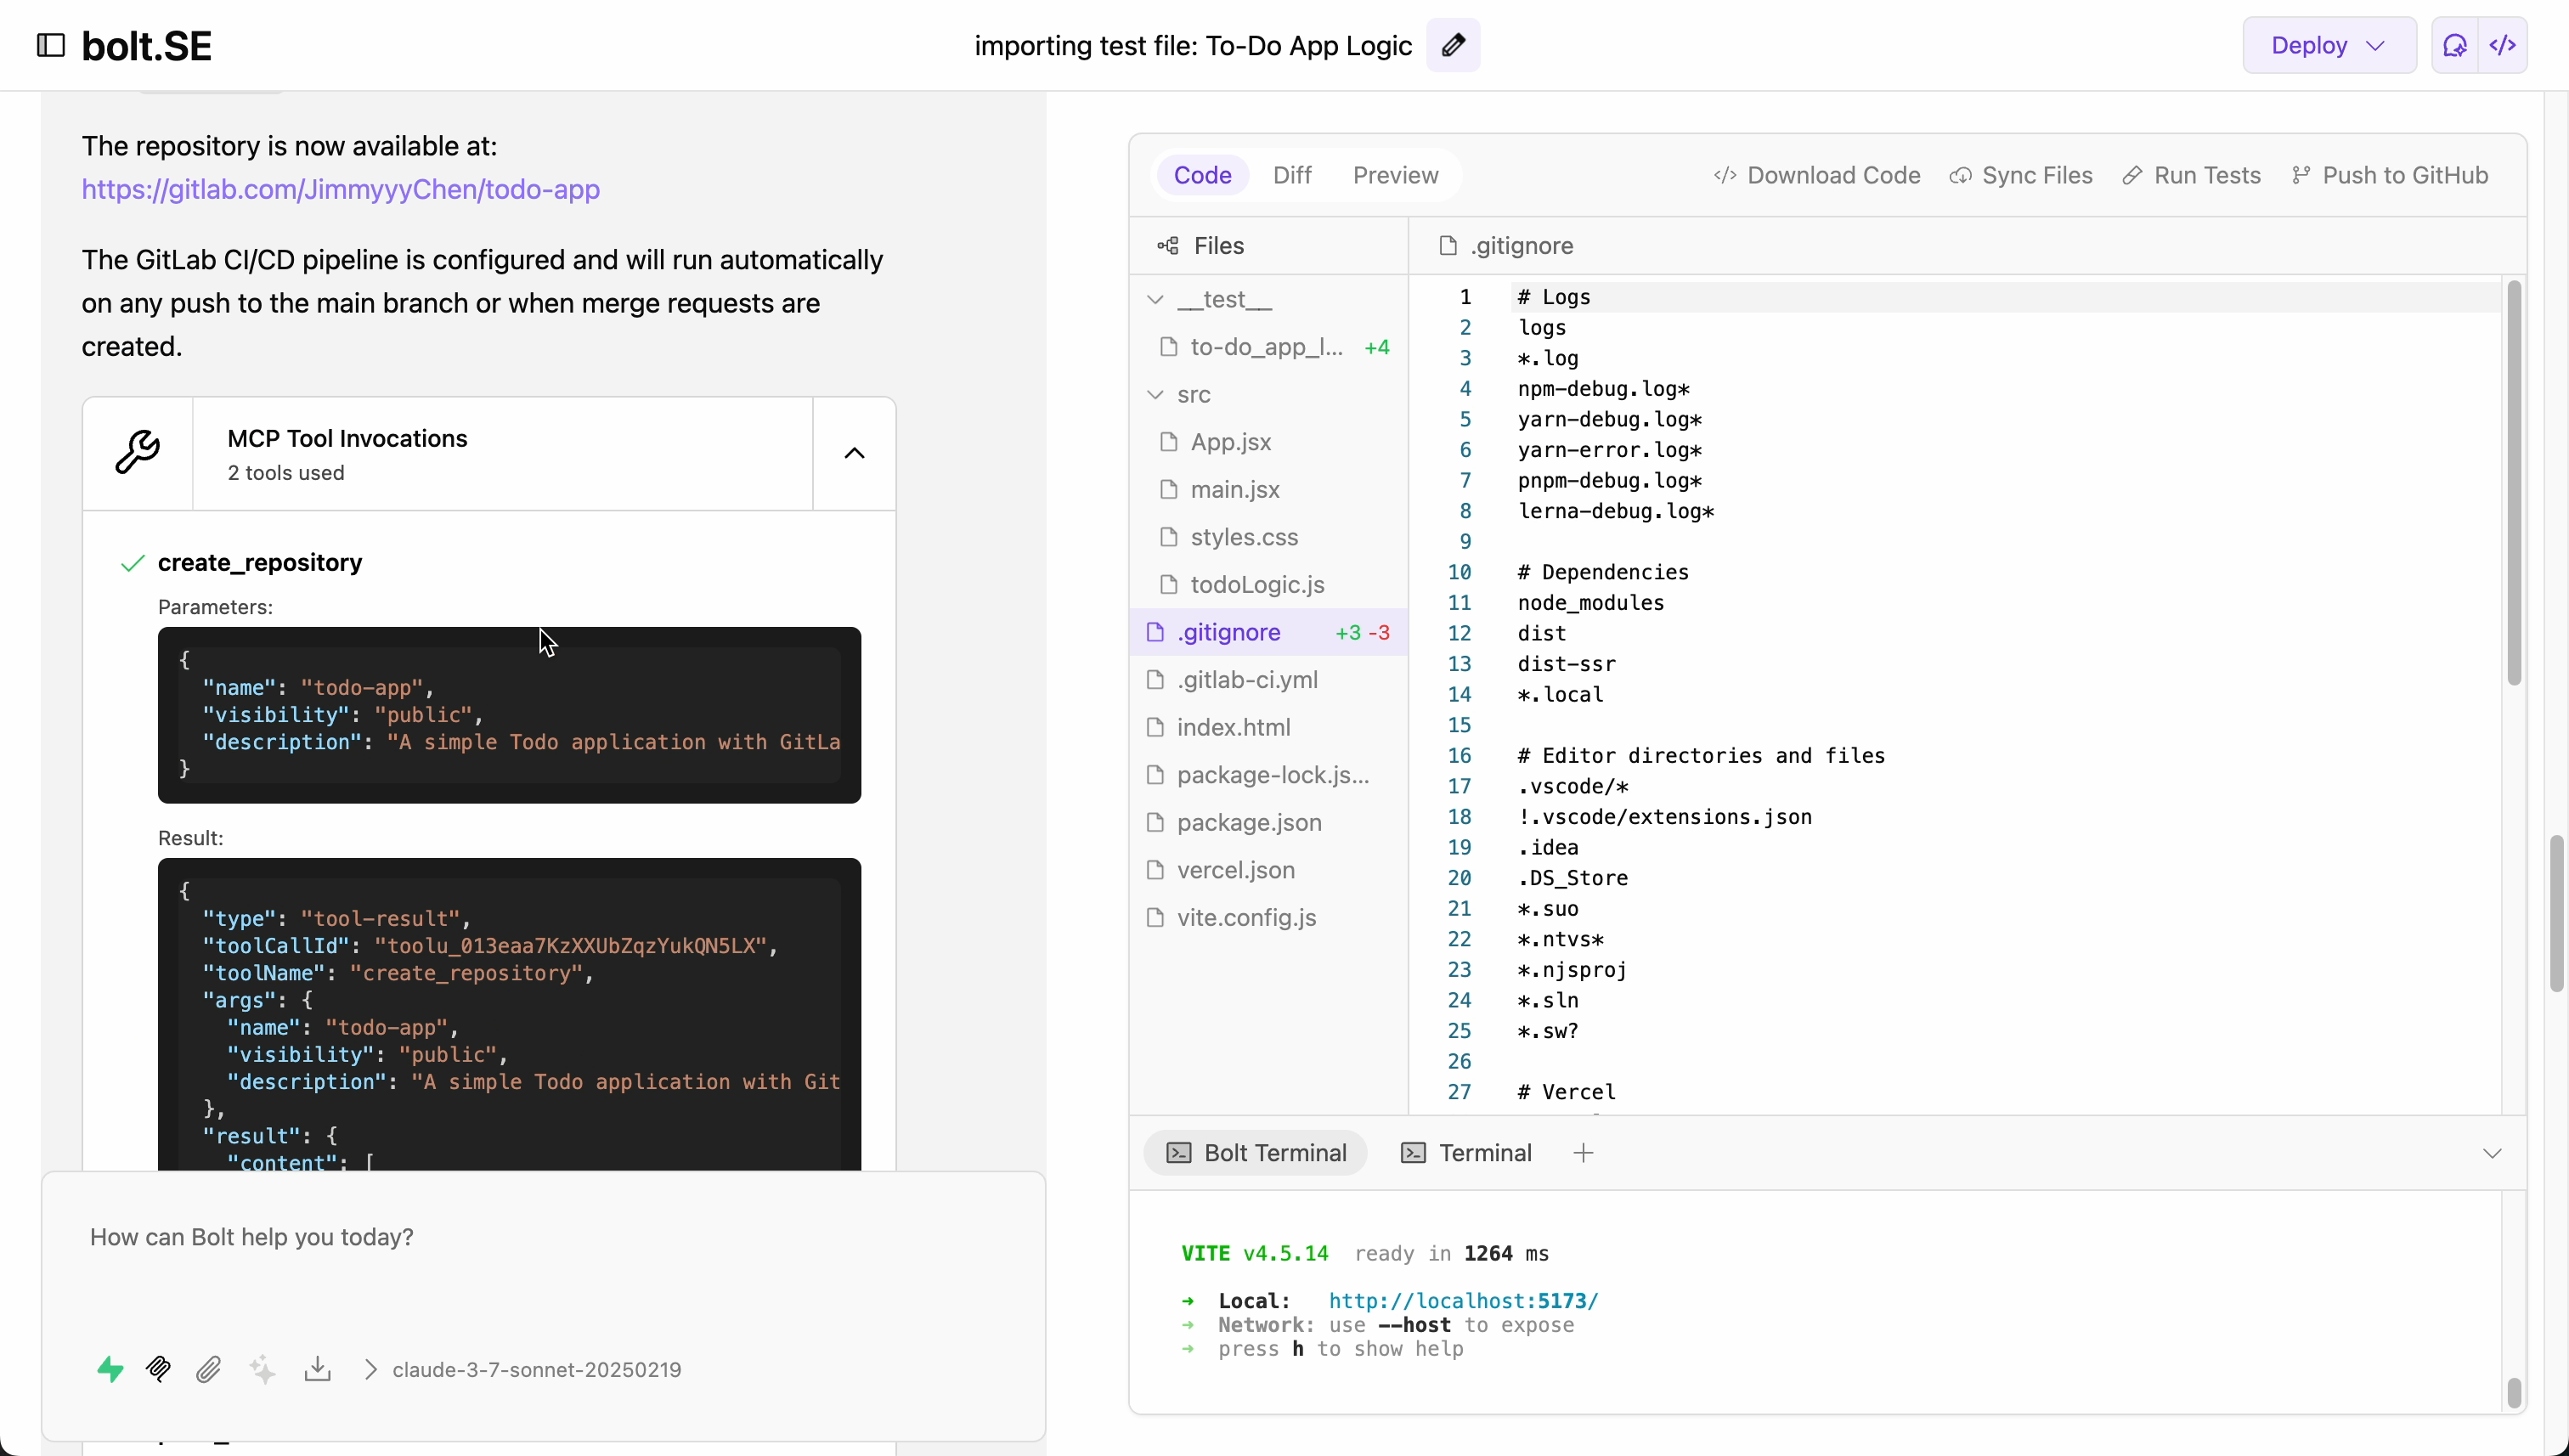
\includegraphics[width=\textwidth]{figures/screenshots/ci-cd/mcp_invocation.png}
  \caption{MCP 工具 \texttt{create\_repository} 的调用参数与返回结果}
  \label{fig:mcp_invocation}
\end{figure}

GitLab 网页端界面(图 \ref{fig:gitlab_repo})可见首个提交 \textit{Add Todo app with GitLab CI/CD and Vercel deployment} 已完成;流水线正在运行,稍后即可在 Vercel 控制台查看部署链接。

\begin{figure}[H]
  \centering
  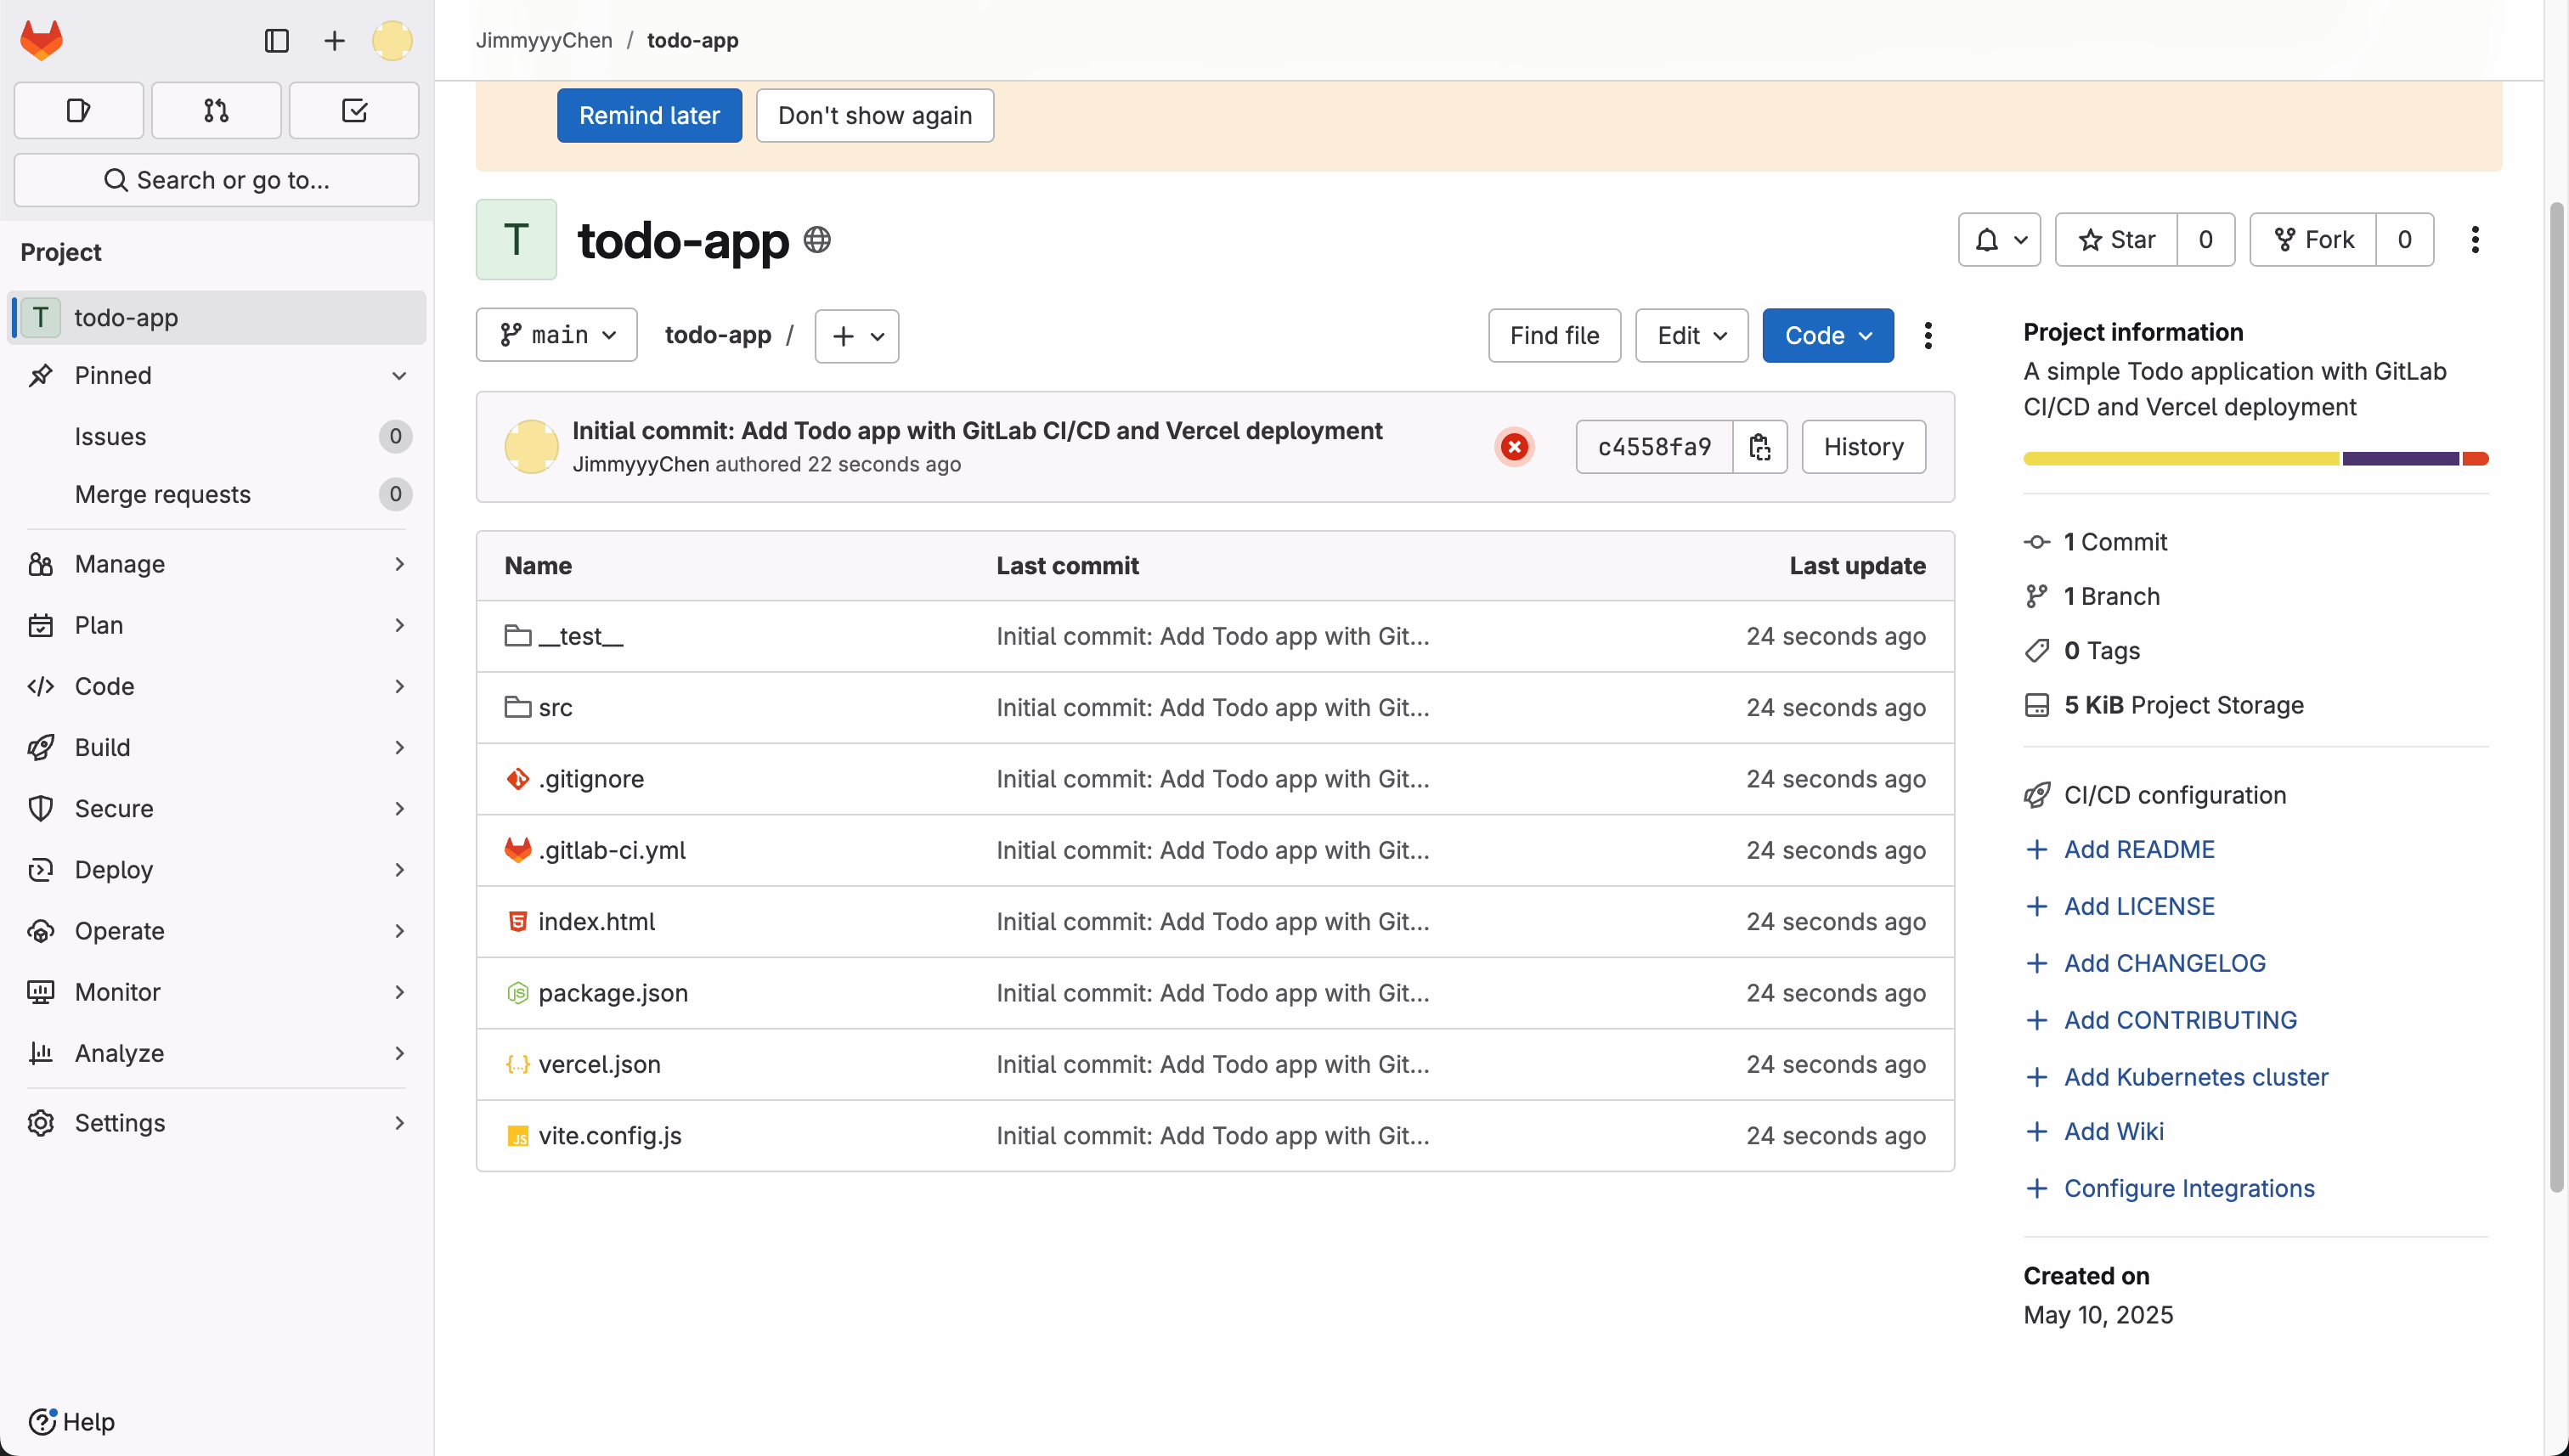
\includegraphics[width=\textwidth]{figures/screenshots/ci-cd/gitlab_repo.png}
  \caption{远端仓库初始化结果(GitLab UI)}
  \label{fig:gitlab_repo}
\end{figure}

通过将 MCP 与 TDD 模块的紧密结合,bolt.SE 实现从本地测试、自动集成到生产部署的完整流程自动化。该案例表明,在完善的测试约束和标准化协议支持下,开发者可以更高效地完成 DevOps 流程,显著减少重复性操作。